\section{Experiments}
\label{sec:experiments}

\subsection{Evaluation Protocol}
\label{sec:dataset_setting}

We evaluate four research questions using two 500-example processed Wikipedia benchmarks, full-wiki HotpotQA, the official 2Wiki split-union corpus and external news validation. Processed pools are jointly indexed but remain question-derived; the corpus-scale indexes are question-independent. The primary processed tier uses MiniLM, while generator comparisons fix BGE-base. Methods, reader interfaces and index sizes are specified in Section~\ref{sec:method}.

Retrieval outcomes are any supporting-title hit@10, all supporting-title hit@10, and mean supporting-title recall@10. We emphasize all-support hit and recall because multi-hop answering can fail when one required page is absent. Reader outcomes are normalized Exact Match (EM) and token F1. The hypothetical passage is used only to form a retrieval query and is never supplied to the reader as evidence. Exact normalized title--paragraph matching, corpus construction, deduplication, top-$k$, and leakage diagnostics are detailed in Online Resource 1, Sections~\SuppRef{sec:supp_deduplication_sensitivity}, \SuppRef{sec:supp_dense_encoder_truncation}, \SuppRef{sec:supp_metric_normalization} and~\SuppRef{sec:supp_answer_overlap_normalization}.

All confirmatory contrasts use paired examples. Effect intervals are question-level percentile bootstrap intervals with 10,000 resamples; binary paired outcomes use exact McNemar tests. Holm correction applies within each stated family. Allowlisted metric exports contain identifiers or their hashes, conditions, scores and provenance, excluding benchmark text and private predictions. Reconstruction coverage and missing inputs are listed separately in Online Resource 1, Section~\SuppRef{sec:supp_code_artifact_availability}.

Hosted results support frozen-artifact audit without an independently verified immutable provider snapshot. The local tiers use pinned weights; IRCoT and four-shot Query2doc-style are disclosed adaptations rather than historical reproductions. Their implementation boundaries are specified in Section~\ref{sec:implementation_boundary} and Online Resource 1.

The transportability axes remain bounded. HotpotQA uses a complete 2017 English Wikipedia index, whereas the 2Wiki corpus is frozen from released benchmark contexts and is not a second complete Wikipedia snapshot. The latter removes question-specific candidate pools and supplies an independent corpus-scale, cross-dataset test, but it does not establish transport to another complete Wikipedia collection or to a non-Wikipedia corpus.

\subsection{RQ1: Controlled Evidence Acquisition}
\label{sec:rq1_controlled_evidence}

The primary predeclared comparison asks whether one document-like expansion improves complete evidence acquisition relative to question-only Dense RAG under the frozen hosted-generator pipeline. On HotpotQA, HyDE raises all-support hit@10 from 0.6300 to 0.8680, a paired difference of $+0.2380$ (95\% CI $[0.2000,0.2780]$), and raises supporting-title recall from 0.8080 to 0.9280 ($+0.1200$; $[0.1010,0.1410]$). Reader EM/F1 increase from 0.5940/0.7199 to 0.6840/0.8105 (Online Resource 1, Section~\SuppRef{sec:supp_hotpotqa_paired_statistics}). This is a positive effect in one frozen hosted artifact, not evidence that the effect is contamination-free or invariant to generator replacement. The secondary 2Wiki check has a positive direction under the same protocol (Online Resource 1, Section~\SuppRef{sec:supp_2wiki_paired_statistics}).

The matched-call mechanism controls show that an additional generation call alone is insufficient. Single-query reformulation remains near the Dense baseline, whereas the hypothetical passage alone reaches 0.8480 all-support hit and question plus hypothetical passage reaches 0.8680. Against question plus rewrite, the latter gains $+0.2400$ ($[0.2020,0.2780]$) in all-support hit and $+0.1250$ ($[0.1060,0.1470]$) in recall (Online Resource 1, Section~\SuppRef{sec:supp_hotpotqa_paired_statistics}). Length-matched, equal-budget, stronger-encoder and top-$k$ diagnostics qualify mechanism attribution (Online Resource 1, Sections~\SuppRef{sec:supp_detailed_sensitivity}, \SuppRef{sec:supp_query_length_matched_hyde}).

Generated benchmark content is part of the main interpretation rather than a peripheral limitation. The fixed lexical/entity classifier assigns the 500 HotpotQA hosted passages to exact-answer, alias/proxy, supporting-entity/title-only, and no-identifiable-gold-content strata in counts of 292/22/154/32. On the original MiniLM artifacts, the 208 answer-absent examples retain a $+0.0620$ reader-F1 difference over Dense ($[0.0170,0.1080]$), and gold-aware answer/title scrubbing retains positive retrieval point estimates. These aggregate controls are not content-free: the answer-absent subset combines the last three strata, while string deletion can leave unrecognized factual proxies.

The fixed four-group contrast holds the hosted passages and BGE-base retriever constant (Online Resource 1, Section~\SuppRef{sec:supp_plan_b_sensitivity}). In the exact-answer stratum, all-support hit@10 changes from 0.8973 to 0.9760, a paired difference of $+0.0788$ ($[0.0445,0.1130]$). In the supporting-entity/title-only stratum the difference is $-0.0065$ ($[-0.0584,0.0455]$), and in the no-identifiable-gold-content stratum it is $-0.1250$ ($[-0.2813,0.0000]$). The alias/proxy stratum has only 22 examples and is explicitly flagged as small. The positive direction therefore does not survive in the no-identifiable-content group under BGE. Together with the MiniLM controls, this makes the hosted result a content-dependent observation whose size and direction also depend on the retriever; it does not isolate a content-independent HyDE effect. A deterministic 200-question-per-dataset check against a question-independent 100k processed corpus preserves the aggregate hosted positive direction, but it is not full Wikipedia and does not remove generated-content dependence.

\noindent\textbf{Answer to RQ1.} The hosted gain is a content-dependent, generator--retriever-conditioned artifact observation. Neither matched calls nor content strata establish a contamination-free mechanism.

\subsection{RQ2: Generator Dependence}
\label{sec:rq2_generator_dependence}

Figure~\ref{fig:generator_contrasts} places the standard hosted and local HyDE contrasts against the same question-only BGE baseline, preserving their original adjusted decisions.

The generator comparison holds BGE-base, serialization, corpus, top-$k$, and the 500 paired questions fixed. On HotpotQA, Dense, Qwen HyDE, and Mistral HyDE obtain all-support hit@10 of 0.882, 0.846, and 0.848 (Online Resource 1, Section~\SuppRef{sec:supp_plan_b_sensitivity}). Mistral versus Dense has a $-0.034$ paired effect ($[-0.064,-0.006]$), but its exact McNemar result does not survive Holm correction ($p=0.1201$). Mistral and Qwen are nearly indistinguishable ($+0.002$; $[-0.024,0.026]$). On 2Wiki, Mistral's point estimate is 0.510 versus Dense's 0.510 ($0.000$; $[-0.032,0.032]$), with no supported separation reported after adjustment; it differs from Qwen by $+0.018$ ($[-0.012,0.048]$). Thus two independently developed, pinned 7B generators both fail to reproduce the hosted gain under the same retriever, while neither open generator dominates the other.

The four-condition Qwen tier gives the same boundary from a broader set of query forms (Online Resource 1, Section~\SuppRef{sec:supp_plan_b_sensitivity}). Standard HyDE and Query2doc-style (4-shot adaptation) are at or below Dense on both datasets, and evidence-only HyDE is lower than standard HyDE on HotpotQA. In contrast, frozen hosted generations under BGE produce all-support hit@10 of 0.920 on HotpotQA and 0.780 on 2Wiki. The current-alias replay has near-zero exact textual agreement with the frozen hosted output but high embedding similarity, demonstrating why hosted evidence is artifact-auditable rather than byte-replayable. These observed generator differences constrain interpretation; they do not identify a causal generator effect.

\begin{figure}[tbp]
\centering
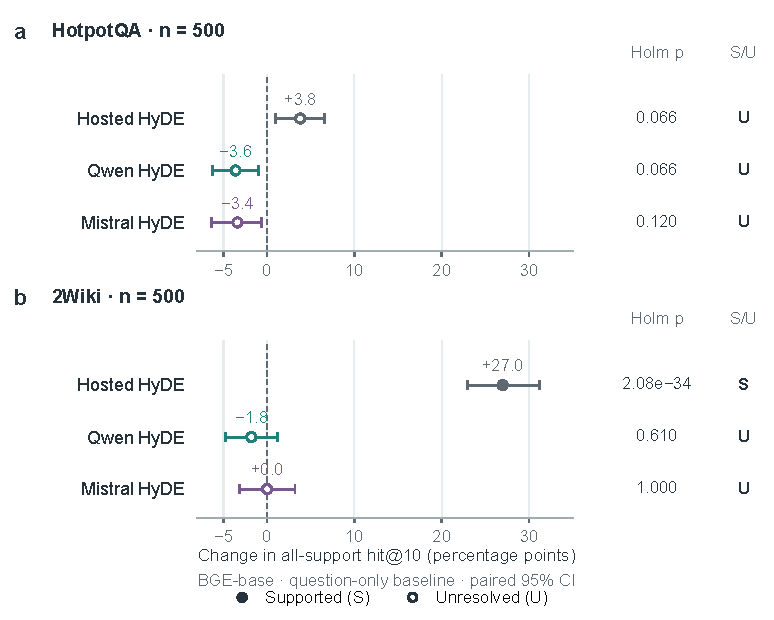
\includegraphics[width=\textwidth]{Fig2_GeneratorContrasts.pdf}
\caption{Generator-conditioned retrieval contrasts. Standard HyDE minus question-only all-support hit@10 with BGE-base on the processed local (a) HotpotQA and (b) 2Wiki corpora, each with 500 questions. Points and bars show paired effects and reported 95\% bootstrap intervals in percentage points. Filled (S) and hollow (U) points preserve supported and unresolved decisions from the original Holm families, not a newly pooled six-row family. All HotpotQA decisions remain unresolved despite intervals excluding zero. Hosted/local differences include implementation and output budgets.}
\label{fig:generator_contrasts}
\end{figure}


The BGE-prefix intervention changes all-support by at most 1.2 percentage points. All four intervals include zero and adjusted McNemar values are at least 0.7183, supplying no supported explanation for the open-generator result (Online Resource 1, Section~\SuppRef{sec:supp_plan_b_sensitivity}).

The evidence hierarchy is therefore three-level: executable pinned-local evidence, an artifact-level hosted positive control, and overlap/answer-absent/scrubbing diagnostics that delimit but do not certify independence from benchmark knowledge.

\noindent\textbf{Answer to RQ2.} The two pinned open generators do not reproduce the hosted positive point-estimate direction. Their mutual contrast and the corrected Mistral-versus-Dense test remain unresolved; this does not rank hosted and open families generally.

\subsection{RQ3: Full-Wiki Retrieval and Reader Robustness}
\label{sec:rq3_fullwiki_reader}

The initial HotpotQA full-wiki comparison tests OneR/BM25, one-generation HyDE-BM25, and official-code IRCoT on one index. Their all-support hit@10 values are 0.298, 0.348, and 0.354 (Table~\ref{tab:ircot_fullwiki_main}). IRCoT improves over OneR by $+0.056$ ($[0.012,0.100]$; Holm-adjusted McNemar $p=0.0369$), but differs from HyDE by only $+0.006$ ($[-0.042,0.056]$; $p=0.8732$). IRCoT averages 2.104 retrieval/generation rounds.

\begin{table*}[t]
\centering
\caption{HotpotQA full-wiki retrieval, serialized evidence, reader outcomes, and structural cost on the same 500 questions. ``Full para.'' requires every complete annotated supporting paragraph to remain after per-document truncation; dashes mark a paragraph-retention audit not repeated for the later learned-reranker row.}
\label{tab:ircot_fullwiki_main}
\scriptsize
\setlength{\tabcolsep}{4pt}
\textbf{A. Retrieval and evidence interface}\par\vspace{2pt}
\begin{tabularx}{\textwidth}{>{\raggedright\arraybackslash}X rrrrr}
\toprule
Condition & All title@10 & Full para. 450 & Full para. 900 & Ret. calls & Query gen. \\
\midrule
OneR/BM25 & 0.298 & 0.112 & 0.288 & 1.000 & 0.000 \\
HyDE-BM25 & 0.348 & 0.102 & 0.332 & 1.000 & 1.000 \\
Official IRCoT + Qwen & 0.354 & 0.140 & 0.340 & 2.104 & 2.104 \\
BM25 + BGE-base rescore & 0.460 & 0.176 & 0.434 & 1.000 & 0.000 \\
BM25 + BGE reranker v2-m3 & 0.468 & -- & -- & 1.000 & 0.000 \\
\bottomrule
\end{tabularx}

\vspace{5pt}
\textbf{B. Frozen evidence under two readers}\par\vspace{2pt}
\begin{tabular}{lrrrr}
\toprule
Condition & Qwen EM & Qwen F1 & Mistral EM & Mistral F1 \\
\midrule
OneR/BM25 & 0.220 & 0.2815 & 0.148 & 0.2674 \\
HyDE-BM25 & 0.236 & 0.3017 & 0.170 & 0.3032 \\
Official IRCoT + Qwen & 0.262 & 0.3366 & 0.160 & 0.2920 \\
BM25 + BGE-base rescore & 0.270 & 0.3469 & 0.186 & 0.3372 \\
BM25 + BGE reranker v2-m3 & 0.264 & 0.3480 & 0.208 & 0.3476 \\
\bottomrule
\end{tabular}
\par\smallskip
\parbox{0.97\textwidth}{\footnotesize Exact title and exact title--paragraph coverage coincide in the four interface-audited rows. Full-paragraph retention is conservative because the aligned artifact lacks official supporting-sentence IDs. Each method has one final reader call. BGE-base is retained as a separately labeled bi-encoder sensitivity comparator; the learned cross-encoder was evaluated with both readers.}
\end{table*}


The registered learned comparator, \texttt{BAAI/bge-reranker-v2-m3}, cross-encodes each question--paragraph pair in the frozen BM25 top-100 pools. It obtains any-hit/all-support/recall of 0.948/0.468/0.708. Its all-support improvements over OneR, HyDE, and IRCoT are $+0.170$ ($[0.136,0.206]$), $+0.120$ ($[0.076,0.162]$), and $+0.114$ ($[0.064,0.164]$); all three paired binary tests remain significant after Holm correction. The earlier BGE-base bi-encoder rescore reaches 0.460 and Qwen EM/F1 of 0.270/0.3469. Its retrieval score is only $0.008$ below the cross-encoder ($[-0.002,0.020]$), so the cross-encoder's advantage over the cheaper bi-encoder is unresolved.

The cross-encoder improves EM over BM25 by $+0.044$ for Qwen ($[0.014,0.074]$; $p_{\mathrm{Holm}}=0.0214$) and $+0.060$ for Mistral ($[0.032,0.090]$; $p_{\mathrm{Holm}}=0.0003$). Table~\ref{tab:ircot_fullwiki_main} preserves absolute EM/F1. Against IRCoT, Qwen EM is unresolved ($+0.002$; $[-0.040,0.042]$), while Mistral gains $+0.048$ ($[0.014,0.082]$). The cross-reader interaction for its BM25 gain is unresolved ($-0.016$; $[-0.046,0.016]$), so supported gains for both readers do not establish invariant effect sizes. Full F1 effects and paired statistics appear in Online Resource 1, Section~\SuppRef{sec:supp_plan_b_sensitivity}.
The earlier reader-by-method interaction remains unresolved: for IRCoT versus HyDE, the Qwen-minus-Mistral interaction is $+0.036$ EM ($[-0.004,0.074]$; exact sign-flip $p_{\mathrm{Holm}}=0.2562$). Reader-specific point estimates therefore do not establish a statistically reliable reader-by-method interaction.

The independent 2Wiki tier gives a narrower corpus-scale result (Table~\ref{tab:2wiki_corpus_scale}). On the 428,395-paragraph split-union corpus, BM25, Qwen-HyDE, IRCoT, and the cross-encoder obtain all-support hit@10 of 0.346, 0.356, 0.342, and 0.400. The cross-encoder has a supported retrieval gain over BM25 of $+0.054$ ($[0.032,0.078]$; $p_{\mathrm{Holm}}=2.23\times10^{-5}$). The verified S1 matrix supports this retrieval contrast on the two tested corpus configurations. HyDE ($+0.010$; $[-0.014,0.032]$) and IRCoT ($-0.004$; $[-0.052,0.042]$) likewise remain unresolved. The cross-encoder's answer gains over BM25 remain unresolved for Qwen (EM $+0.014$; $[-0.016,0.044]$) and Mistral (EM $+0.008$; $[-0.012,0.028]$). The observed retrieval increase is therefore configuration-specific and does not support a cross-dataset answer-superiority claim.

\begin{table*}[t]
\centering
\caption{Transport check on the independent split-union corpus frozen from the official 2Wiki release. The corpus-scale tier is not a second complete Wikipedia snapshot.}
\label{tab:2wiki_corpus_scale}
\scriptsize
\setlength{\tabcolsep}{3pt}
\resizebox{\textwidth}{!}{%
\begin{tabular}{lrrrrrr}
\toprule
Method & All-support@10 & Recall@10 & Qwen EM & Qwen F1 & Mistral EM & Mistral F1 \\
\midrule
BM25 OneR & 0.346 & 0.671 & 0.212 & 0.224 & 0.052 & 0.164 \\
Qwen-HyDE & 0.356 & 0.665 & 0.186 & 0.209 & 0.056 & 0.162 \\
IRCoT + Qwen & 0.342 & 0.654 & 0.218 & 0.246 & 0.072 & 0.185 \\
BGE reranker v2-m3 & 0.400 & 0.705 & 0.226 & 0.244 & 0.060 & 0.172 \\
\bottomrule
\end{tabular}
}
\end{table*}


Scorer/adapter sensitivity and official-code stopping deviations, including the retained hard-cap row, are documented in Online Resource 1, Sections~\SuppRef{sec:supp_metric_normalization} and~\SuppRef{sec:ircot_fullwiki}.

\noindent\textbf{Answer to RQ3.} Cross-encoder retrieval gains are supported on both corpus-scale tiers, but answer gains are supported for both readers only on HotpotQA. Both 2Wiki answer decisions remain unresolved.

\subsection{RQ4: IRCoT Round-Budget Sensitivity}
\label{sec:rq4_round_budget}

The round-prefix analysis asks how the frozen IRCoT trajectory changes after one round, after two rounds, and at its natural or capped exit. It is a sensitivity analysis, not a strict equal-budget comparison: later prefixes contain more retrieved documents and more generation calls, and questions may stop at different rounds. From round 1 to round 2, all-support hit rises from 0.158 to 0.344 ($+0.186$; $[0.152,0.220]$), EM from 0.166 to 0.254 ($+0.088$; $[0.062,0.116]$), and F1 by $+0.0981$ ($[0.0710,0.1264]$). Holm-adjusted exact tests remain significant for retrieval ($p<10^{-27}$) and EM ($p<10^{-9}$); the complete round table appears in Online Resource 1.

The increment from round 2 to the full trajectory is much smaller: all-support increases by $+0.010$ ($[0.002,0.020]$), EM by $+0.008$ ($[0.002,0.016]$), and F1 by $+0.0077$ ($[0.0017,0.0154]$). The corresponding adjusted exact tests are not significant ($p=0.0625$ for all-support and $p=0.125$ for EM). Most measured benefit therefore arrives by the second round under this configuration, whereas later adaptive continuation has a small average point gain. One retained hard-cap example and its post-hoc sentence-boundary sensitivity are documented in Online Resource 1, Section~\SuppRef{sec:ircot_fullwiki} and do not alter aggregates.

\noindent\textbf{Answer to RQ4.} Most observed gain arrives by round two under unequal accumulated cost; this does not establish an optimal stopping rule.

\subsection{External News-Corpus Validation: MultiHop-RAG}
\label{sec:mhrag_external}

MultiHop-RAG~\cite{tang2024multihoprag} supplies a news-document benchmark outside the Wikipedia-oriented tiers. The complete frozen release has 2,556 questions: retrieval and answer EM/F1 use 2,255 non-null questions; 301 null queries define separate canonical abstention. Support is matched by parent-document evidence IDs, rather than Wikipedia titles. Five available retrieval methods, two pinned readers and both 450/900-character evidence settings yield 20 sealed cells with 51,120 answers.

This is an available-condition analysis, not a complete six-condition transfer test. IRCoT is technically unavailable because the frozen local adapter assumes the HotpotQA corpus/index and lacks registered external parser, prompt, stopping and smoke anchors. This limits the implementation, not the IRCoT algorithm. Four observed contrasts versus BM25 use Holm correction with a fifth slot reserved conservatively at 1.0; no observed IRCoT $p$-value is imputed. The full registered family and transport decision are not complete.

% Generated by scripts/build_jiis_chatfix_tables.py; available evidence only.
\begin{table*}[!htbp]
\centering\footnotesize
\caption{MultiHop-RAG retrieval on 2,255 non-null queries (top-10).}
\label{tab:mhrag_retrieval}
\begin{threeparttable}
\setlength{\tabcolsep}{3pt}
\begin{tabular}{lrrrrlr}
\toprule
Method & Any & All & Recall & $\Delta$All & 95\% CI & $p_{\rm Holm}$ \\
\midrule
BM25 & 0.982 & 0.583 & 0.807 & -- & -- & -- \\
Dense BGE & 0.979 & 0.503 & 0.767 & -0.079 & [-0.098, -0.060] & $<0.001$ \\
Qwen-HyDE & 0.970 & 0.448 & 0.731 & -0.134 & [-0.155, -0.114] & $<0.001$ \\
Mistral-HyDE & 0.968 & 0.434 & 0.718 & -0.149 & [-0.169, -0.128] & $<0.001$ \\
Cross-encoder & 0.996 & 0.729 & 0.890 & +0.146 & [+0.127, +0.165] & $<0.001$ \\
\bottomrule
\end{tabular}
\begin{tablenotes}\scriptsize\item Parent-document evidence IDs define support; 301 null queries are excluded from retrieval denominators. Cross-encoder reranks a frozen BM25 top-100 pool. All-support and EM are primary endpoints. Four observed contrasts versus BM25 use Holm correction with a fifth slot conservatively reserved at 1.0 for unavailable IRCoT; this is not an observed IRCoT $p$-value. The full registered family is incomplete. Intervals are 95\% question-level bootstrap intervals (10,000 resamples); intervals alone do not determine significance.
\end{tablenotes}
\end{threeparttable}
\end{table*}


Complete-support retrieval is \MHRBMAll{} for BM25, \MHRDenseAll{} for Dense, \MHRQAll{} for Qwen-HyDE and \MHRMAll{} for Mistral-HyDE. All three adjusted contrasts with BM25 are negative. The cross-encoder reaches \MHRCEAll{}, with a positive adjusted gain of \MHRCEGain{} (Table~\ref{tab:mhrag_retrieval}). Standard open-generator expansion therefore supplies no observed gain over the lexical baseline here, while reranking the frozen BM25 top-100 pool does.

New post-hoc comparisons also match each expansion directly to the same Dense baseline on all 2,255 non-null IDs. All-support deltas are $-0.0550$ for Qwen-HyDE and $-0.0692$ for Mistral-HyDE, with Holm-adjusted $p=2.29\times10^{-11}$ and $3.24\times10^{-17}$. All eight reader/length EM comparisons favor Dense after adjustment. These additional families leave the historical BM25 family unchanged (Online Resource 1, Section~\SuppRef{sec:supp_priority_diagnostics}).

Retrieval improvement only partly carries through to answers. Cross-encoder EM gains over BM25 are positive after adjustment with both readers at 450 characters and Qwen at 900 characters; Mistral/900 remains unresolved. Both HyDE variants have negative adjusted EM contrasts with Qwen at both lengths; their Mistral contrasts are unresolved. Dense improves Mistral/900 EM, with the other EM contrasts unresolved. The exploratory EM interaction is significant only for Mistral-HyDE versus BM25 at 450 characters. Non-significant interactions do not establish reader invariance. Both lengths, secondary F1, raw/adapted scores and null abstention are retained in supplementary Section~\SuppRef{sec:supp_mhrag_external} in Online Resource 1.

Figure~\ref{fig:retrieval_answer_contrasts} summarizes the cross-encoder contrasts with BM25 across the three corpus-scale evaluations. Retrieval gains are supported in each, whereas the answer decisions depend on corpus, reader and, for news, character budget. The distinct support definitions and endpoints preclude a pooled gain or retrieval-to-answer conversion rate.

\begin{figure}[tbp]
\centering
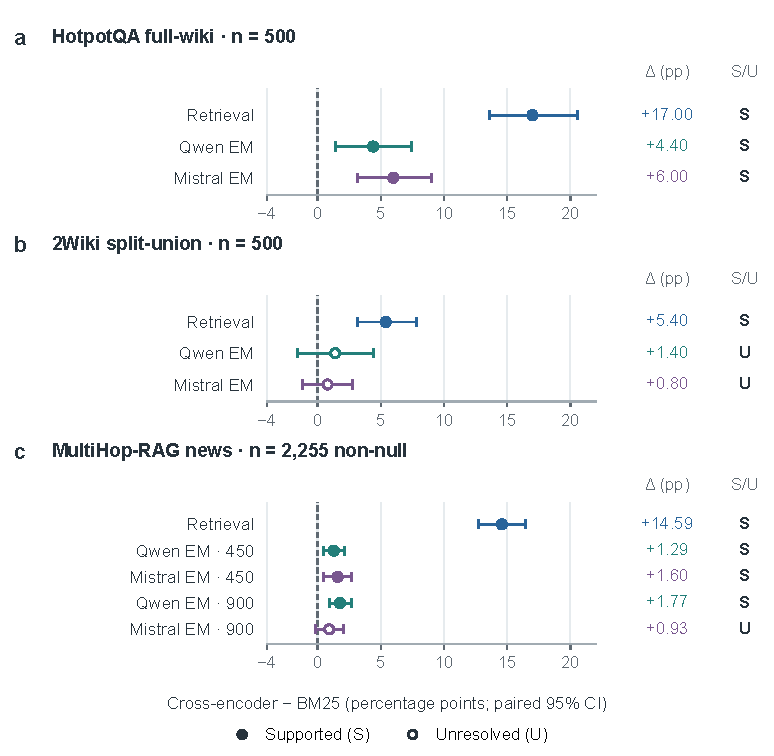
\includegraphics[width=\textwidth]{Fig3_RetrievalAnswer.pdf}
\caption{Retrieval and answer gains across evaluated configurations. Cross-encoder minus BM25 paired effects and reported 95\% bootstrap intervals on (a) HotpotQA full-wiki, (b) 2Wiki split-union and (c) MultiHop-RAG news. Retrieval is all-support hit@10; answer quality is exact match (EM). News labels 450/900 denote characters per document; retrieval is drawn once. Filled (S) and hollow (U) points preserve original Holm decisions. Wiki support uses titles; news support uses parent-document evidence IDs and excludes 301 null questions. Effects are not pooled across endpoints or corpora and do not estimate causal mediation.}
\label{fig:retrieval_answer_contrasts}
\end{figure}


Null queries expose a separate reader limitation. Mistral/900 canonical abstention is 0.0299 for both BM25 and the cross-encoder, compared with Qwen at 0.6611/0.6213. However, lexical refusal expressions occur in 170/301 and 153/301 Mistral outputs, respectively. This gap and frequent output-cap termination indicate a format-sensitive endpoint, rather than a human-confirmed hallucination rate. The registered adapter and canonical-null scores remain unchanged.

On the frozen 500-question prompt subset, query2doc-style improves all-support retrieval over standard for both generators after adjustment; evidence-only does not. Same-subset Dense and BM25 scores are 0.502 and 0.590, versus 0.516/0.512 for Qwen/Mistral Query2doc-style. The new 36-contrast post-hoc family leaves both Query2doc-versus-Dense comparisons unresolved and both contrasts with BM25 negative. Seed dispersion on the disjoint 300-question subset remains descriptive; alternative-prompt answer gains are unmeasured. Missing end-to-end costs prevent efficiency claims, and withdrawn independent human validation leaves evidence sufficiency unmeasured.


\subsection{Evidence-Interface Audit}
\label{sec:evidence_interface_audit}

Figure~\ref{fig:evidence_retention} distinguishes retrieved supporting titles, retained annotated sentences and retained full paragraphs under two character budgets. The original frozen-label audit has title and annotated-paragraph completeness coinciding before serialization. At 450 characters, complete paragraphs remain verbatim for 0.112/0.102/0.140/0.176 of questions for OneR, HyDE, IRCoT and BGE-base; at 900 characters the rates are 0.288/0.332/0.340/0.434 (Table~\ref{tab:ircot_fullwiki_main}).

The retrospective official-sentence audit uses the same 500 IDs and retains all annotated sentences for 0.254/0.284/0.298/0.388 of questions at 450 characters (Online Resource 1, Table~\SuppRef{tab:supporting_sentence_audit}). One official supporting-title set differs from the frozen labels; Figure~\ref{fig:evidence_retention} consistently uses official labels and preserves the primary results.

A final-input audit includes the learned cross-encoder and both reader templates on these 500 IDs. All 5,000 actual 450-character inputs remain below 2,000 tokens, with reconstructed prompts matching stored hashes. Cross-encoder annotated-sentence completeness falls from 0.470 at retrieval to 0.390 after character serialization, with no further token-stage loss. The other methods retain 0.254/0.284/0.298/0.388 under both readers. Historical effective-token hashes were not recorded, so inputs are reconstructed. The earlier 500-question 900-character audit is counterfactual; actual matched-budget answers are reported below. Retention does not establish factual sufficiency (Online Resource 1, Section~\SuppRef{sec:supp_priority_diagnostics}).

\begin{figure}[tbp]
\centering
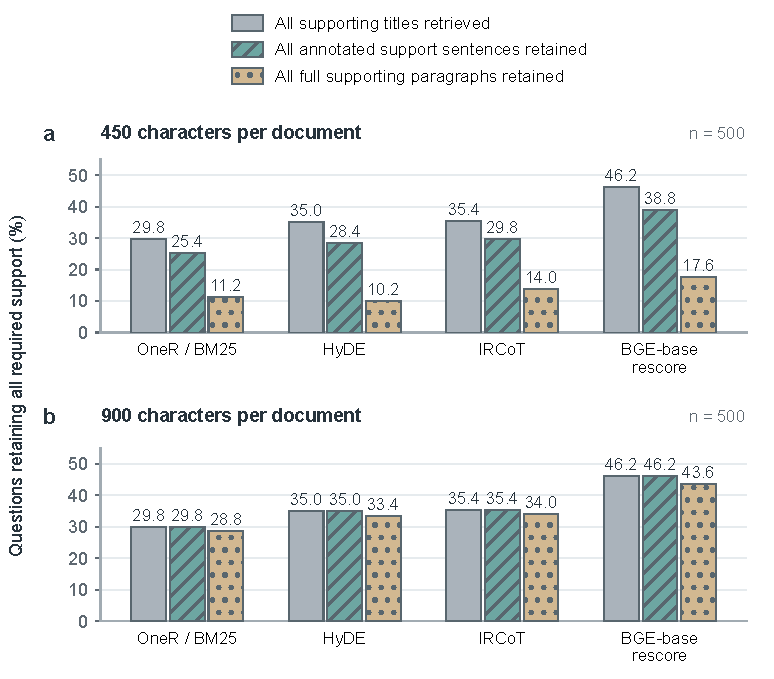
\includegraphics[width=\textwidth]{Fig4_EvidenceRetention.pdf}
\caption{Annotated evidence retention under (a) 450 and (b) 900 characters per document. Bars show complete-support question rates on 500 frozen HotpotQA IDs using the official retrospective sentence-audit labels consistently: all supporting titles retrieved, all annotated sentences retained and all full supporting paragraphs retained. One official title set differs from the primary labels; original scores remain unchanged (Online Resource 1, Section~\SuppRef{sec:supp_sentence_audit}). BGE-base rescore is a bi-encoder, distinct from Figure~\ref{fig:retrieval_answer_contrasts}. Coverage precedes global token clipping and does not establish human sufficiency. Bars are descriptive.}
\label{fig:evidence_retention}
\end{figure}


A matched intervention then generates 400 fresh answers on the first 100 original questions with fixed cross-encoder evidence, comparing 450 and 900 characters under the same suffix-preserving input policy. Complete support retention rises from 46\% to 55\%, with no token-stage clipping. Qwen EM remains 0.29 ($\Delta=0$; 95\% CI $[-0.05,0.05]$); Mistral changes from 0.22 to 0.21 ($\Delta=-0.01$; $[-0.06,0.03]$). Neither EM nor F1 establishes a gain: both separately specified two-test families have adjusted $p=1$ for each reader. Increased annotated-support delivery therefore does not guarantee improved answer scores in this diagnostic. Actual token amounts differ; it is neither an equal-cost comparison nor independent validation (Online Resource 1, Section~\SuppRef{sec:supp_followup_serializer}).

\subsection{Reader Controls and New-sample Validation}
\label{sec:new_reader_controls_results}
On the fixed 100-question subset, Qwen EM is 0.09 without supplied evidence and 0.57 with complete gold-selected support. Historical same-ID BM25/cross-encoder EM is 0.18/0.29. Mistral gives 0.05/0.35 without evidence/with gold support, versus 0.15/0.22 for BM25/cross-encoder. Local and official EM coincide for these comparisons, although F1 conventions differ.

Gold support improves Qwen EM over the cross-encoder by $+0.28$ [$0.18,0.38$], with adjusted $p=1.36\times10^{-5}$. Mistral's $+0.13$ [$0.02,0.24$] remains unresolved after adjustment ($p=0.0702$). The ten-contrast EM family includes both readers and all five fixed comparisons per reader. Gold-selected support improves both readers over question-only, yet neither reaches perfect EM. These controls expose remaining benchmark-answer errors without assigning them uniquely to reasoning, formatting or retrieval. Full outputs and termination diagnostics appear in Online Resource 1, Table~\SuppRef{tab:priority_reader_controls}.

A separate 64-question dev check excludes all 500 previously observed project IDs. The frozen retrieval-mean and audit-informed rules both select the cross-encoder before new outcomes. Shared selected-policy EM is 0.2813 for Qwen and 0.2188 for Mistral. Complete annotated support falls from 33/64 retrieved to 24/64 after character serialization, with no additional token loss. The identical choices yield structural zero performance increment, with no inferential test or general method-selection advantage (Online Resource 1, Section~\SuppRef{sec:supp_independent_validation_new}).

\subsection{Implementation and Validation Synthesis}
\label{sec:implementation_validation_synthesis}

The named local contrasts (Table~\ref{tab:boundary_stability_matrix}) support reranker retrieval over BM25 in the tested HotpotQA and 2Wiki configurations; 2Wiki answer gains remain unresolved. A deterministic reporting-rule analysis of 32 unique observed primary effects gives 19 favorable and 13 adverse point estimates, versus 12 supported, seven rejected and 13 unresolved effects using their original Holm families (Online Resource 1, Table~\SuppRef{tab:claim_stress}). Seven favorable point estimates remain unresolved after correction. This is descriptive re-expression, without new tests or a measure of framework accuracy. Five unavailable external IRCoT slots are excluded from observed counts; they still constrain transport. Framework positioning from primary papers is reported in Online Resource 1, Table~\SuppRef{tab:framework_comparison}.

\subsection{Complete Comparison on Random New Questions}
\label{sec:followup_holdout_results}
The new 300-question full-wiki matrix (Online Resource 1, Section~\SuppRef{sec:supp_followup_holdout}) runs all three methods under both readers. Complete-support retrieval is 0.350/0.440/0.537 for BM25/HyDE/CE; all three paired improvements are supported. CE-minus-BM25 EM is $+0.090$ for Qwen (CI $[0.050,0.130]$, $p_{\mathrm{Holm}}=0.000152$) and $+0.070$ for Mistral ($[0.030,0.110]$, $p=0.003764$). HyDE-minus-BM25 EM is supported for Qwen ($+0.060$, $p=0.011740$) and unresolved for Mistral ($+0.0167$, $p=0.499560$). CE-minus-HyDE EM is unresolved for Qwen and supported for Mistral; both secondary F1 contrasts are supported. These local decisions do not test a reader interaction. Complete annotated support reaches actual input in only 86/103/121 questions, with no further token-stage loss. New means remain separate from historical results and use the official single answer; same-source random new IDs do not establish contamination-free or cross-dataset validation.

\subsection{Failure Analysis and Artifact Availability}
\label{sec:failure_analysis}

Online Resource 1, Table~\SuppRef{tab:evidence_completeness_buckets_supp} separates answers by support completeness, while Table~\SuppRef{tab:single_annotator_error_taxonomy} describes retrieval, reasoning and surface-form errors. The latter is a single-annotator diagnostic, not a validated annotation benchmark; full case records and qualitative examples are reported in Online Resource 1, Sections S16--S17.

The allowlisted capsules reconstruct summary tables, eight historical open-generator retrieval contrasts and all 31 new serializer/holdout contrasts. Missing inputs still limit news reanalysis, raw-prediction rescoring and model reruns; full boundaries appear in Online Resource 1, Section~\SuppRef{sec:supp_code_artifact_availability}.
